\documentclass{www2009-submission}

\usepackage[cp1250]{inputenc}  % or [cp1250], or [latin2], or whatever
                               % suitable for your system

\begin{document}
%
\title{Web Semantization}

\numberofauthors{3}

\author{
\alignauthor Jan Dedek\\
       \affaddr{Department of Software Engineering}\\
       \affaddr{Charles University in Prague}\\
       \affaddr{Malostranske namesti 25 }\\
       \affaddr{Prague, Czech Republic}\\
       \email{jan.dedek@mff.cuni.cz}
\alignauthor Alan Eckhardt\\
       \affaddr{Institute of Computer Science, Academy of Sciences of the Czech Republic}\\
       \affaddr{Pod Vodarenskou vezi 2}\\
       \affaddr{Prague, Czech Republic}\\
       \email{eckhardt@cs.cas.cz}
\alignauthor Peter Vojtas\\
       \affaddr{Institute of Computer Science, Academy of Sciences of the Czech Republic}\\
       \affaddr{Pod Vodarenskou vezi 2}\\
       \affaddr{Prague, Czech Republic}\\
       \email{vojtas@cs.cas.cz}
}

\maketitle
\begin{abstract}
Web Semantization is a concept we introduce in this paper. We understand Web Semantization as an automated process of increasing degree of semantic content on the web. Part of content of the web is further usable, semantic content (usually annotated) is more suitable for machine processing.
The idea is supported by models, methods, prototypes and experiments with a web repository, automated annotation tools producing third party semantic annotations, semantic repository serving as a sample of semantized web and a proposal of an intelligent software agent. We present a proof of concept that even today it is possible to develop a semantic search engine designed for software agents.
\end{abstract}

\category{H.3.1}{INFORMATION STORAGE AND RETRIEVAL}{Content Analysis and Indexing}
\category{H.3.3}{INFORMATION STORAGE AND RETRIEVAL}{Information Search and Retrieval}
\category{I.2.4}{ARTIFICIAL INTELLIGENCE}{Knowledge Representation Formalisms and Methods}

\terms{Web Semantization}

\keywords{Semantic Web, Web Content Mining, Linguistic Analysis}

\section{Introduction}

\begin{figure}[b!]
\centering
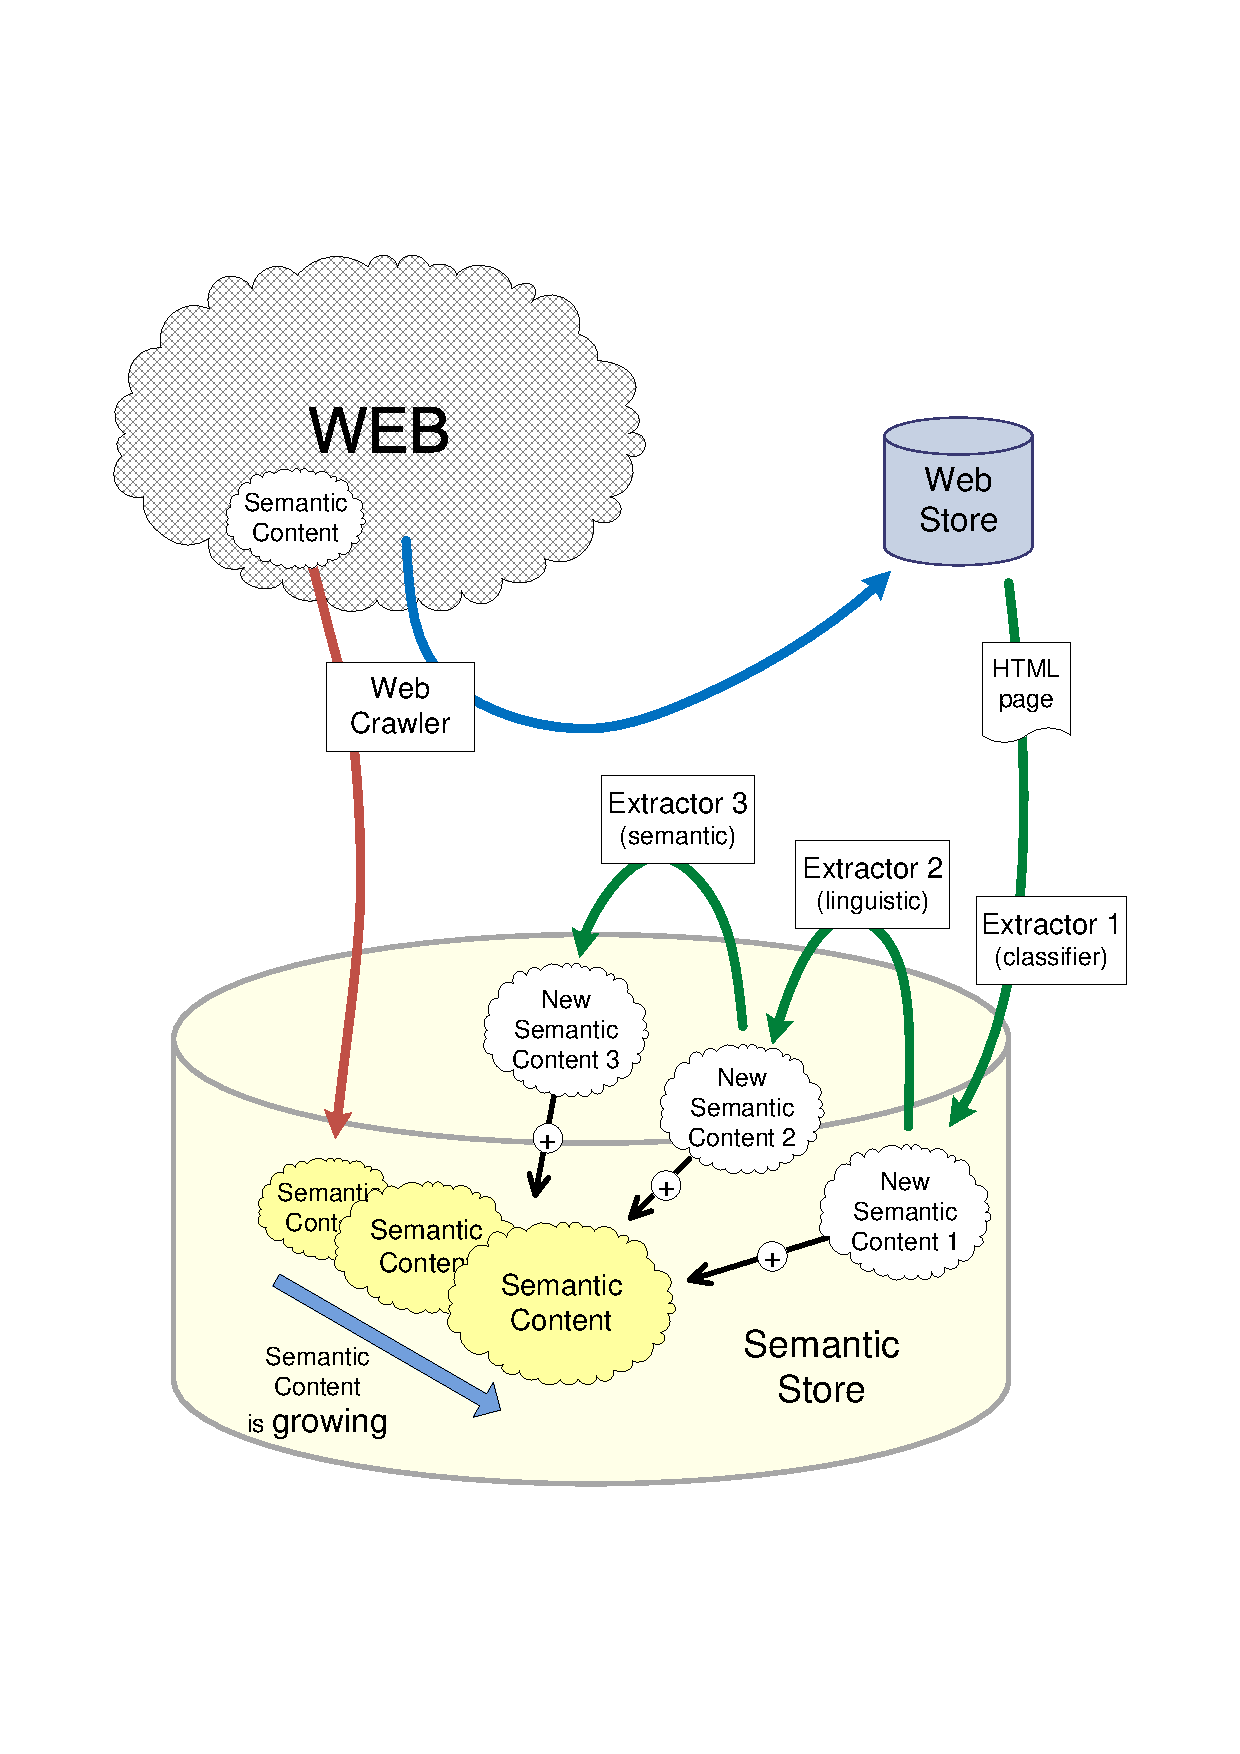
\includegraphics[height=.8\hsize, width=\hsize]{img/Semantization}
\caption{The process of semantization of the Web}
\label{img:Semantization}
\end{figure}

In their Scientific American 2001 article \cite{biblio:2001-Berners-Lee-SemanticWeb}, Tim Berners-Lee, James Hendler and Ora Lassila unveiled a nascent vision of the semantic web: a highly interconnected network of data that could be easily accessed and understood by a desktop or handheld machine. They painted a future of intelligent software agents that would ``answer to a particular question without our having to search for information or pore through results'' (quoted from \cite{biblio:feigenbaum_semantic_2007}). Lee Feigenbaum, Ivan Herman, Tonya Hongsermeier, Eric Neumann and Susie Stephens in their Scientific American 2007 article \cite{biblio:feigenbaum_semantic_2007} conclude that ``Grand visions rarely progress exactly as planned, but the Semantic Web is indeed emerging and is making online information more useful as ever''. L. Feigenbaum et al. support their claim with success of semantic web technology in drug discovery and health care (and several further applications). These are mainly corporate applications with data annotated by humans. Ben Adida when bridging clickable and Semantic Web with RDFa (\cite{biblio:AdidaClickable}) assumes also human (assisted) activity by annotations of newly created web resources. \par

But what to do with the content of the web of today or of pages published without annotations? The content of the web of today is too valuable to be lost for emerging semantic web applications. We are looking for a sulution how to make it accessible in semantic manner. \par

In this paper we would like to address the problem of semantization (enrichment) of current web content as an automated process of third party annotation for making at least a part of today's web more suitable for machine processing and hence enabling it intelligent tools for searching and recommending things on the web (see \cite{biblio:LeeWebThings}). \par

Our main idea is to fill a semantic repository with information that is automatically extracted from the web and make it available to software agents. We give a proof of concept that this idea is realizable and we give results of several experiments in this direction.

Our web crawler (see Fig.\ref{img:Semantization}) downloads a part of the web to the web repository (Web Store). Resources with semantic content can be uploaded directly to the semantic repository (Semantic Store). Extractor~1 (classifier) extracts those parts of Web Store which are suitable for further semantic enrichment (we are able to enrich only a part of resources). More semantic content is created by several extractors and annotators in several phases. The emphasis of this paper is on the automation and the usage of such extracted/enriched data.


\section{Idea of Web semantization}
%Here we would like to present the idea of our contribution to web semantization.

\textbf{First idea is the idea of a web repository.} It develops as follows in details. Semantic enrichment is in fact a data mining task (although a special one) - to add to web documents a piece of knowledge, which is obvious for human perception not for a machine. That means to annotate data by concepts from an ontology which is the same as to map instances to ontology. Such a data mining task will be easier to solve when there is a sort of a repetition (modulo some similarity).\par 
We decided to enrich only textual content for the present, no multimedia (this substantially reduces the size of information we have to store). Especially we restrict to the pages with content consisting either dominantly of grammatical sentences (let us call them textual pages) and those containing large number of table cells (let us call them tabular pages). Of course this division need not be disjoint, and will not cover the whole web. 


%\subsection{Web repository}
The Web repository is a temporal repository of Web documents crawled by a crawler. The repository supports document's metadata, e.g. modification and creation dates, domain name, ratio HTML code/text, content type, language, grammatical sentences etc. It keeps track of all changes in a document and simplifies access to and further processing of Web documents. We are experimenting with the Web crawler Egothor\footnote{http://www.egothor.org/} 2.x and it's Web repository. We have been filled this repository with several terabytes of textual part of Czech web (domain *.cz) and it very simplified access to this data.

%The architecture is based on three layers: core that saves documents and computes deltas between revisions to save space; symlink that maps core's document and revision numbers to numbers published to a user; cloud that assigns tags and manages ACL on the tags. This way the system can modify the tags without overloading the main base of raw documents.

%, so that it is able to provide information about a durable (persistent) text blocks or even subtrees in DOM.


%To be able to separate durable grammatical or table pages poses special requirements to search in our web repository.\par

\textbf{Second idea is to split annotation process to two parts}, one domain independent intermediate annotation and second domain dependent user directed annotation. Both should be automated, with some initial human assisted learning. This first part of learning could require assistance of a highly skilled expert; the second (probably faster part) should be doable by an user with average computer literacy. \par

The first domain independent annotation will serve as an intermediate annotation supporting further processing. This will run once on the whole suitable data. Hence initial necessary human assistance in training can be done by a highly skilled expert (indeed it can be a longer process).\par
The second domain dependent annotation part can consists of a large number of tasks with different domains and ontologies. This should be possible to be executed very fast and if possible with assistance of an average computer skilled user.  We can afford this having intermediate annotation. \par


\textbf{Domain independent intermediate annotation} can be done with respect to general ontologies. First ontology is the general PDT tectogrammatical structure \cite{biblio:MiBeAnnotationtectogrammatical2006} (it is not exactly an ontology written in ontology language, but could be considered this way) which captures semantic meaning of a grammatical sentence. This is the task for computational linguistics; we make use of their achievements which were originally focused on machine translation. Of course tectogrammatical structure is not the only option for this purpose. English language for example can be parsed in many different ways (most often according to some kind of grammar). All the other possibilities are applicable, but in our current solution we make use of a tree structure of the annotations. In this paper we will present our experience with Czech language and tectogrammatical structure that we have used for domain independent intermediate annotation of pages dominantly consisting of grammatical sentences. 

For structured survey or product summary pages (we call them ``tabular pages'') we assume that their structure is often similar and the common structure can help us to detect data regions and data records and possibly also attributes and values from detailed product pages. Here annotation tools will be also trained by humans -- nevertheless only once for the annotation of the whole repository.

%We have identified two types of web resources where this can be done. The first are "table pages", containing large number of cells with abbreviated description of a resource and corresponding detailed pages. Here we assume that content of cells is similar and content of detailed pages is also similar. Because of space limitations, we do not describe our approach for these pages.

%The second are pages dominantly consisting of grammatical sentences. Thanks to the fact that we have a third party linguistic tool for the creation of tectogrammatical trees of sentences, this can be done without requirement of similarity repetition. This situation is illustrated in the Fig.~\ref{fig:similarity}.

We can see an interesting inversion in the use of similarity and repetition. %depicted in Fig.~\ref{fig:similarity}.

While for tabular pages we use similarities in the intermediate phase, for textual pages we use similarities in the domain dependent phase where similar sentences often occur.


%\begin{figure}
%\label{fig:similarity}
%\begin{center}
%\begin{tabular}{|p{100pt}||p{100pt}|p{100pt}|} \hline
%Type of annotation&Tabular pages&Textual pages\\ \hline\hline
%Intermediate general&Uses similarities&Does not use similarities\\ \hline
%Domain dependent&Does not use similarities&Uses similarities\\ \hline
%\end{tabular}	
%\end{center}
%\caption{Use of similarity in annotation approaches}
%\end{figure} 

\textbf{Domain (task) dependent (on demand) annotation} is concerning only pages previously annotated by general ontologies. This makes second annotation faster and easier. An assistance of a human is assumed here for each domain and new ontology. For textual pages repetitions make possible to learn a mapping from structured tectogrammatical instances to an ontology. This domain (task) dependent task can be avoided by a collaborative filtering method, assuming there is enough users' acquaintance. \par

Third important idea is to \textbf{design semantic repository}. It should store all the semantic data extracted by extraction tools and accessed thorough a semantic search engine. Of course many different problems (e.g. querying and scalability) are connected with this but they are at least partially solved now days. Let us mention work of our colleges \cite{biblio:DoTySemanticWeb2007} that is available for use.

The semantic repository should also contain some sort of uncertainty annotation besides above mentioned ontologies. The main reason is that annotation process is error prone and we can have in future different alternative annotation tools and aggregate results. This aspect is not further described in the paper but can be found with many details in \cite{biblio:DeEcDiscussionUncertainty2008} and \cite{biblio:EcHoUncertaintyIssues2008}.\par

Last, but also important idea is \textbf{(4) to design at least one agent} which will give evidence that our semantization really improved general web search. Besides using annotated data it should also contain some user dependent preference search capabilities.


\begin{figure}
\centering
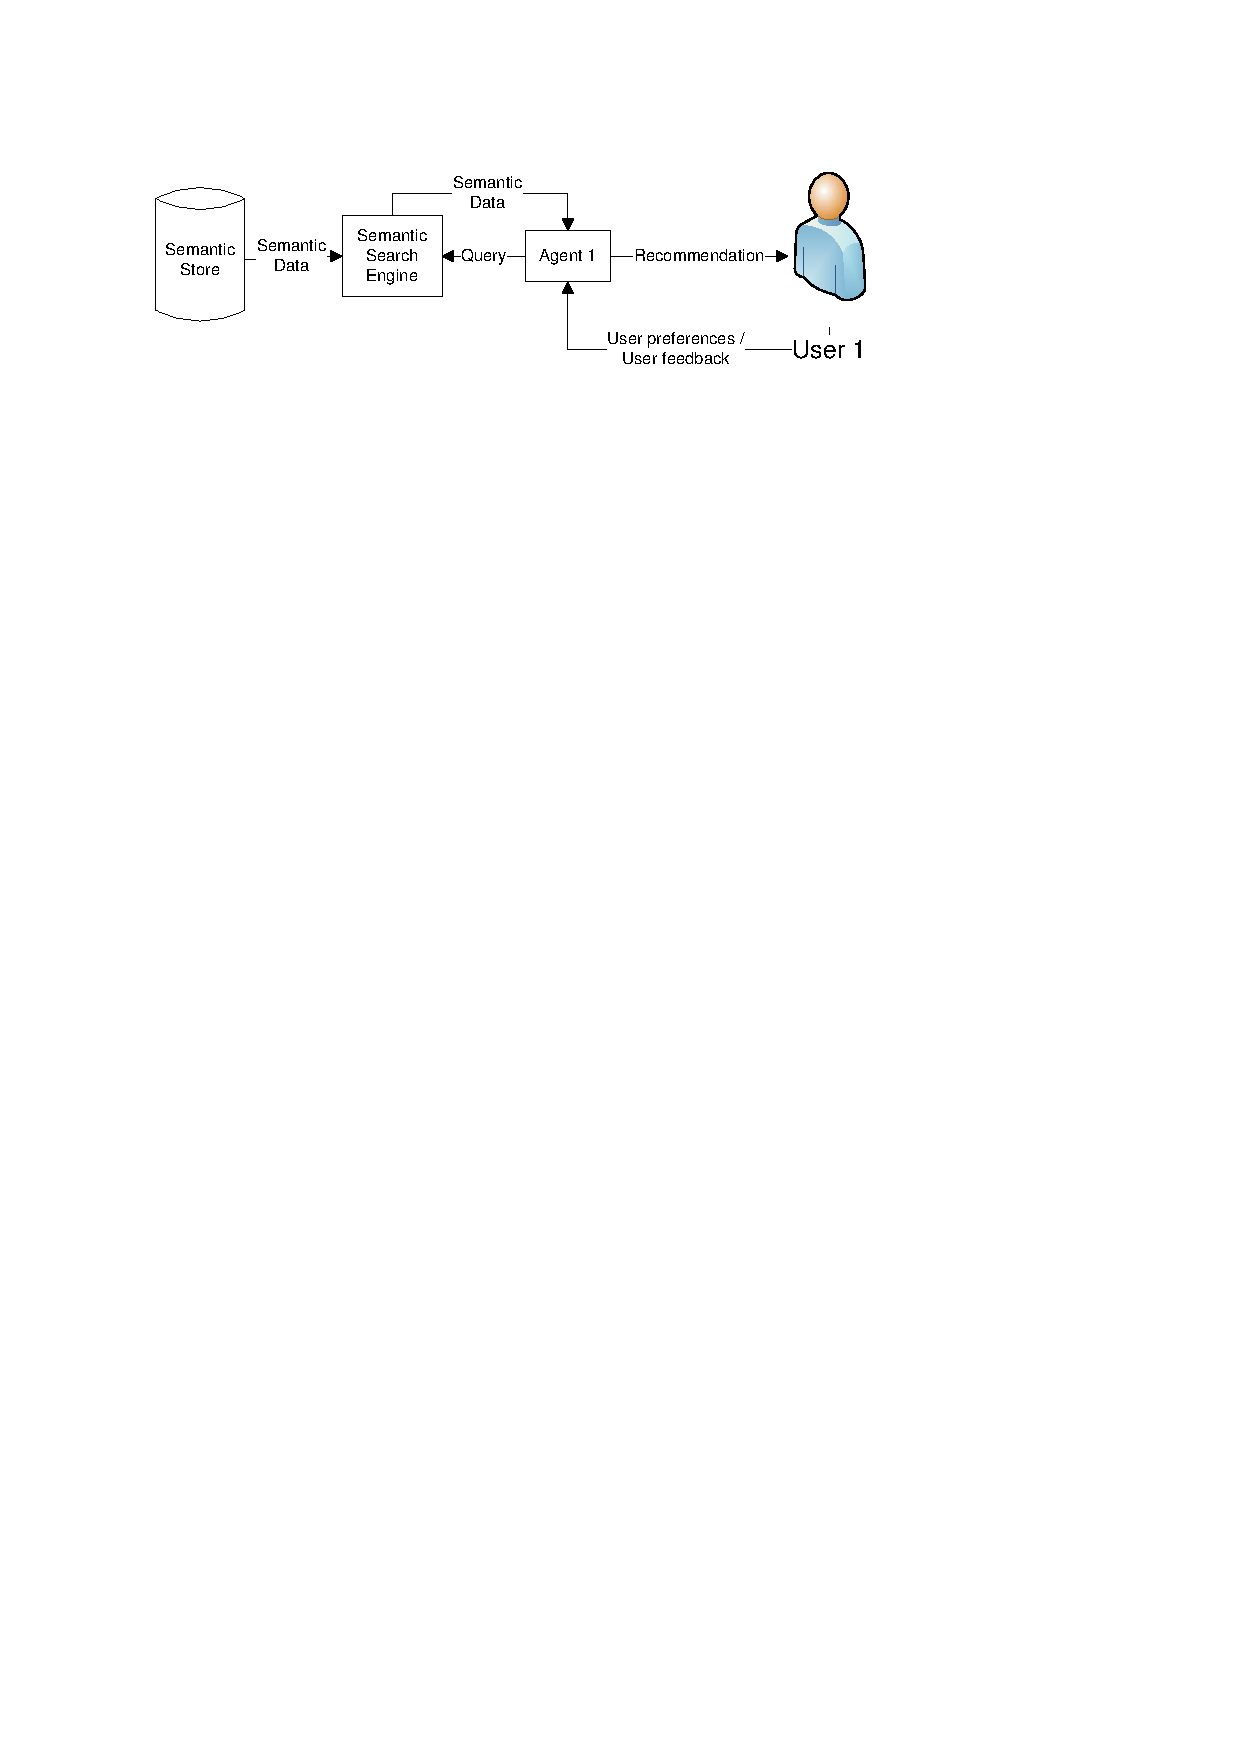
\includegraphics[width=\hsize]{img/UserSearch}
\caption{Process of querying Semantic Search Engine by an user agent}
\label{img:UserSearch}
\end{figure}
 
The process of a user agent searching and making use of semantic search engine is represented in Figure \ref{img:UserSearch}.

Our main focus in this paper is on the agent and on the extractors.


\begin{figure}
\centering
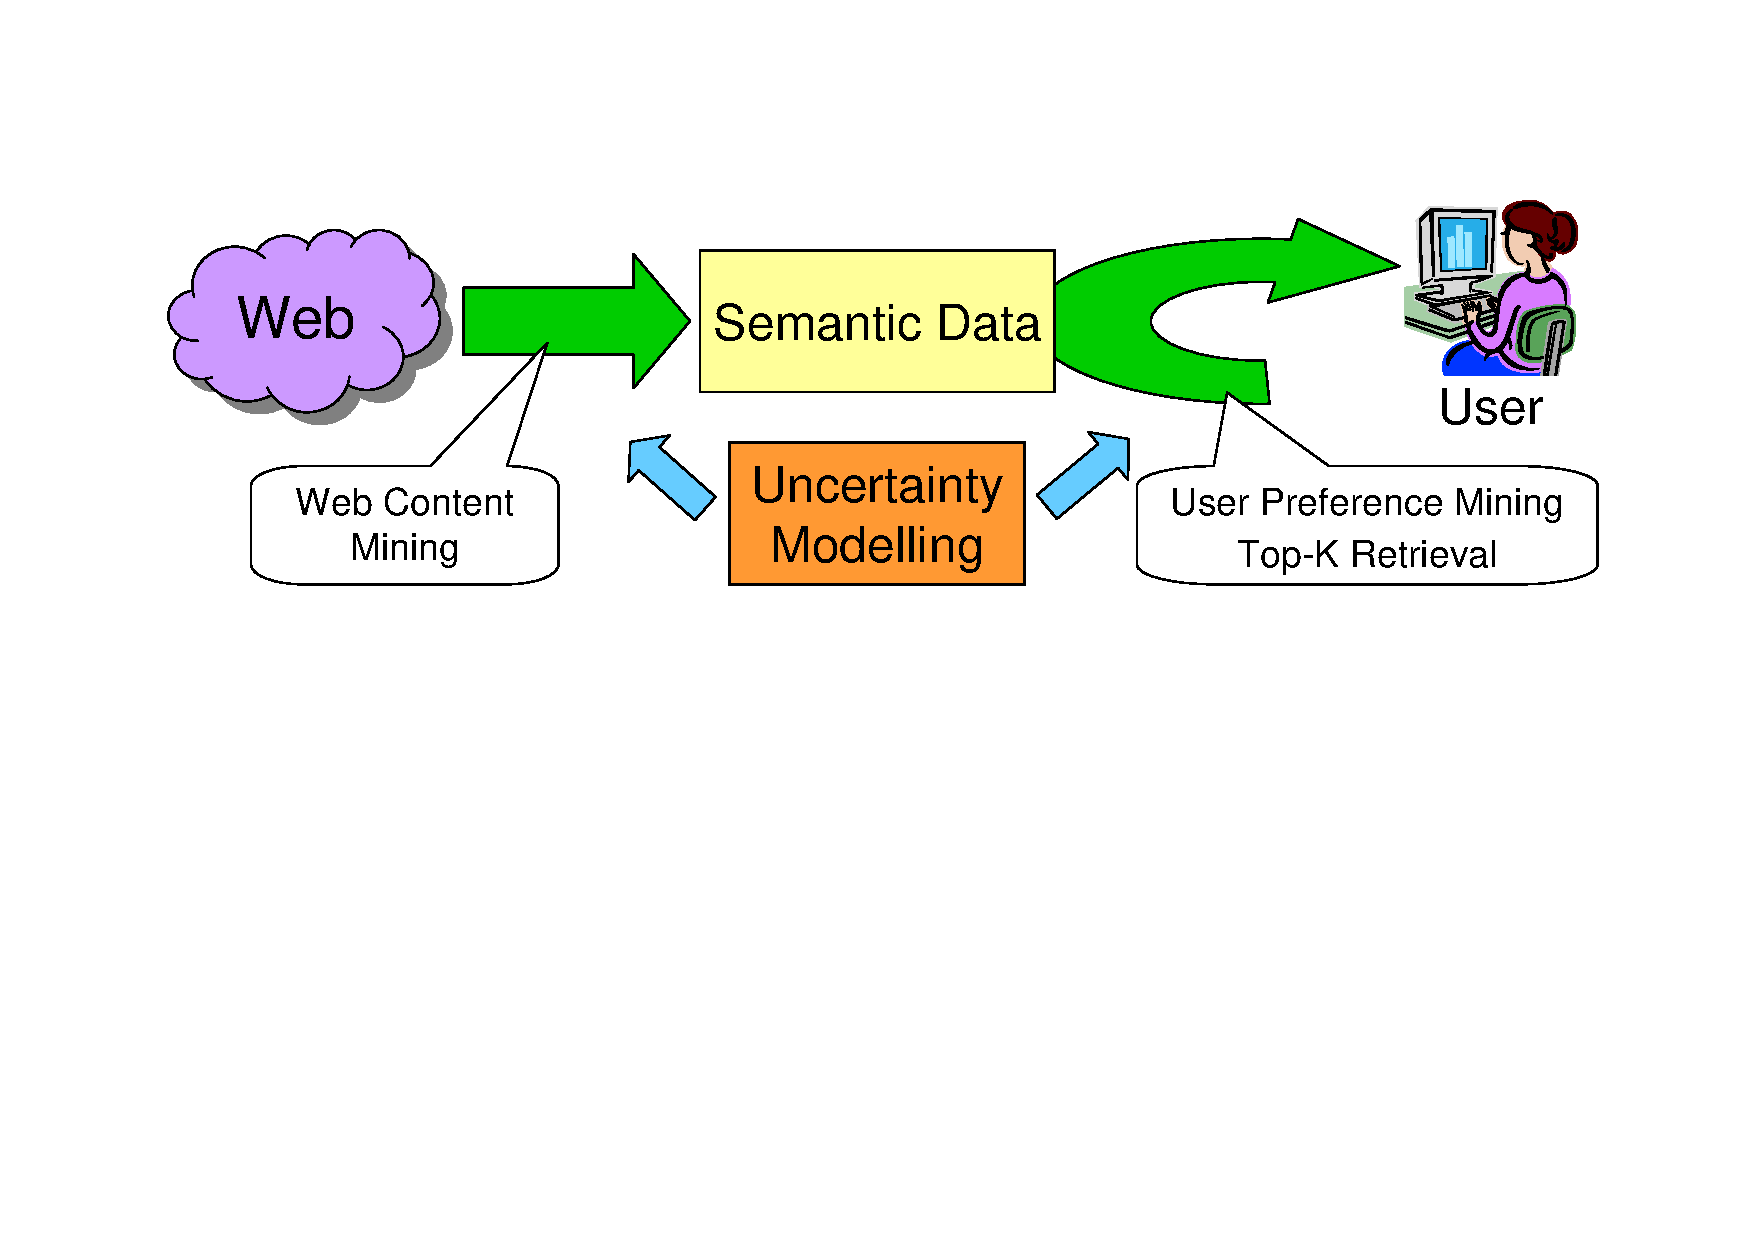
\includegraphics[width=\hsize]{img/Web2User}
\caption{Connecting Web and User}
\label{img:Web2User}
\end{figure}

\begin{figure}
\centering
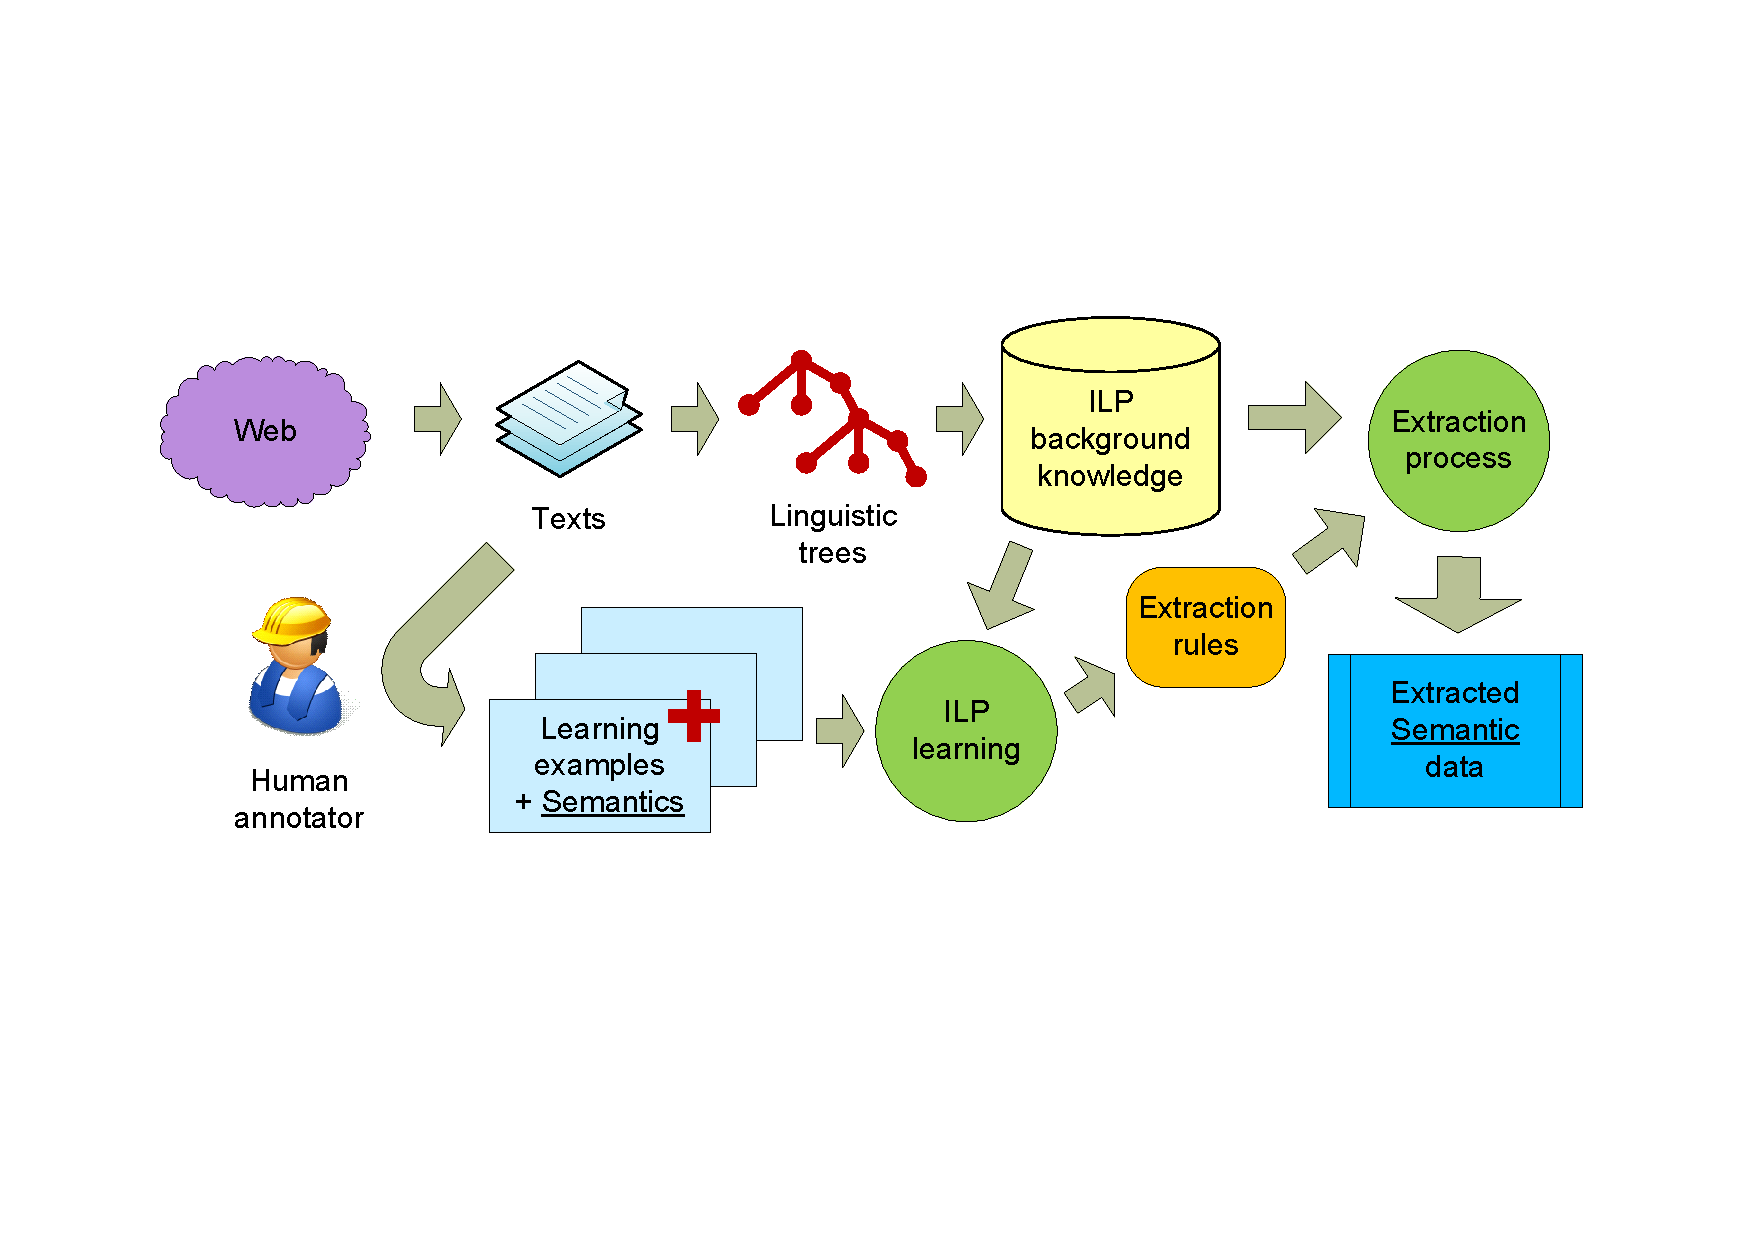
\includegraphics[width=\hsize]{img/DedVoj_ILP}
\caption{ILP Learning of Extraction Rules}
\label{img:DedVoj_ILP}
\end{figure}


%ACKNOWLEDGMENTS are optional
\section{Acknowledgments}
This work was partially supported by Czech projects 1ET100300517, 201/09/0990 GACR and MSM-0021620838.

%
% The following two commands are all you need in the
% initial runs of your .tex file to
% produce the bibliography for the citations in your paper.
\bibliographystyle{abbrv}
\bibliography{DedEckVoj_www2009}

\balancecolumns % GM July 2000
% That's all folks!
\end{document}
